%%%%%%%%%%%%%%%%%%%%%%%%%%%%%%%%%%%%%%%%%%%%%%%%%%%%%%%%%%%%%%%%%%%%%%%%%%%%%%%%%%%%%%%%%%
%%
%% Description:		This is an example presentation using the beamerthemedhbw
%%
%%					The beamerthemedhbw is based on jacksbeamertheme
%%					(https://github.com/JacknJo/jacksbeamertheme)
%%
%% Author:			Hannes Bartle																				
%% 					DHBW Ravensburg Campus Friedrichshafen		
%%					September 2016	
%% 
%% The beamerthemedhbw is free software: you can redistribute it and/or modify
%% it under the terms of the GNU General Public License as published by
%% the Free Software Foundation, either version 3 of the License, or
%% (at your option) any later version.
%% 
%% The beamerthemedhbw is distributed in the hope that it will be useful,
%% but WITHOUT ANY WARRANTY; without even the implied warranty of
%% MERCHANTABILITY or FITNESS FOR A PARTICULAR PURPOSE.  See the
%% GNU General Public License for more details.
%% 
%% You should have received a copy of the GNU General Public License
%% along with the beamerthemedhbw.  If not, see <http://www.gnu.org/licenses/>.
%% 
%% 
%%%%%%%%%%%%%%%%%%%%%%%%%%%%%%%%%%%%%%%%%%%%%%%%%%%%%%%%%%%%%%%%%%%%%%%%%%%%%%%%%%%%%%%%%%


\documentclass[	12pt, 				
				t,					
				aspectratio=169,
				%handout-PLACEHOLDER
				]{beamer}

\usepackage{dhbwstyle}

\title{Listenstrukturen}

\begin{document}
	
	\begin{frame}[noframenumbering]
		\titlepage
	\end{frame}


	\begin{frame}[allowframebreaks]{Inhalt}
		\tableofcontents
	\end{frame}
	
	\outlineFrame{Allgemeines}
	\begin{frame}{Multithreading}{Allgemeines (Vgl. \cite{ullenboom2018java} S. 948)}
    \begin{itemize}
        \item Moderne Betriebssysteme unterstützen \textit{Multitasking}
        \item Bedeutet: Mehrere Programme können gleichzeitig laufen
        \item Man spricht in der Regel von \textit{Nebenläufigkeit}
        \item Wie diese erreicht wird steuert das Betriebssystem (und ggf. Hardware)
        \item Auf Mehrkernprozessoren können "`echt parallel"' arbeiten
        \item Auf Einkernsystemen wird eine Parallelität "`simulisert"' (\textit{Quasiparallelität})
    \end{itemize}
\end{frame}

\begin{frame}{Multithreading}{Technische Umsetzung (Vgl. \cite{ullenboom2018java} S. 948)}
    \begin{itemize}
        \item Jeder Prozessorkern kann (in der Regel) zu einem Zeitpunkt einen Prozess bearbeiten
        \item In der Regel gibt es deutlich mehr laufende Prozesse als Kerne
        \item Lösung: Aktiver Prozess wird auf den Kernen hochfrequent (im Millisekundenbereich) umgeschalten
        \item Umschaltung erfolgt durch den \textit{Scheduler}
        \item Zur Umschaltung der Prozesse gibt es diverse Strategien mit diversen Parametern:
        \begin{itemize}
            \item Priorität
            \item Bearbeitungsdauer
            \item "`Fail-Count"' -- Wie oft wurde der Prozess schon versucht zu bearbeiten
        \end{itemize}
    \end{itemize}
\end{frame}

\begin{frame}{Prozesse}{Grundlegende Eigenschaften (Vgl. \cite{ullenboom2018java} S. 948)}
    \begin{itemize}
        \item Jeder Prozess besteht im Grunde aus:
        \begin{itemize}
            \item Dem auszuführenden Programmcode
            \item Den dazugehörigen Daten
            \item Einem \textit{eigenen} (isolierten) Speicherbereich
            \item Ggf. Verwendete Ressourcen wie Dateien oder Laufwerke
        \end{itemize}
        \item Durch die Trennung des Speicherbereichs können Prozesse nicht auf die Daten anderer Prozesse zugreifen!
        \item Ist doch ein Datenaustausch zwischen Prozessen erforderlich, ist ein spezielle \textit{Shared Memory} Bereich notwendig
        \item Prozesse können aus mehreren parallelen Threads bestehen $\rightarrow$ Diese können die gleichen Ressourcen nutzen
    \end{itemize}
\end{frame}

\begin{frame}{Nebenläufigkeit}{Geschwindigkeitsgewinn (Vgl. \cite{ullenboom2018java} S. 949ff)}
    \begin{itemize}
        \item Nebenläufigkeit führt in der Regel zu Geschwindigkeitsgewinn
        \item In Mehrkernsystemen sowieso...
        \item ...aber auch in Einkernsystemen
        \item Beispiel: Software zur Erstellung von Datenbank-Reports:
        \begin{itemize}
            \item Baue ein Fenster auf
            \item Öffnen der Datenbank vom Server, lesen der Datensätze
            \item Analyse der Daten, Visualisierung des Fortschritts
            \item Datei öffnen, Analyseergebnisse in Datei schreiben
        \end{itemize}
    \end{itemize}
\end{frame}

\begin{frame}{Nebenläufigkeit}{Beispiel für Geschwindigkeitsgewinn (Vgl. \cite{ullenboom2018java} S. 949ff)}
    \begin{itemize}
        \item Betrachten wir einmal die parallelisierbaren Abschnitte:
        \begin{itemize}
            \item Öffnen von Fenster und Datenbank können parallel geschehen
            \item Lesen neuer Datensätze und Analyse alter Datensätze kann parallel erfolgen
            \item Analyse neuer Datensätze und schreiben von alten analysierten Daten kann gleichzeitig abgearbeitet werden
        \end{itemize}
        \item Hier auch auf einem Einprozessorsystem großer Leistungsgewinn
        \item Da die parallelen Prozesse verschiedene \textit{Ressourcen} belasten
    \end{itemize}
\end{frame}

\begin{frame}{Nebenläufigkeit}{Beispiel für Geschwindigkeitsgewinn (Vgl. \cite{ullenboom2018java} S. 949ff)}
    \begin{itemize}
        \item Während auf das Fertigstellen einer Ressource gewartet wird, können Aufgaben bearbeitet werden die andere Ressourcen benötigen:
        \begin{itemize}
            \item Während der Prozessor ausgelastet ist die GUI zu erstellen kann eine Datei auf der Festplatte geöffnet werden $\rightarrow$ Dateioperationen benötigen wenig Prozessorleistung, eher durch Festplattengeschwindigkeit begrenzt
            \item Während Daten z.B. aus einer Datenbank abgerufen werden wird hauptsächlich die Netzwerkressource belastet $\rightarrow$ Prozessorleistung kann ggf. anders genutzt werden
            \item Parallel zu einer Prozessorlastigen Analyse können bereits analysierte Daten in eine Datei geschrieben werden
        \end{itemize}
        \item Kurz gesagt: Wir nutzen "`Wartezeiten"' von langsamen Operationen zu unserem Vorteil
    \end{itemize}
\end{frame}

\begin{frame}{Nebenläufigkeit}{Fazit (Siehe \cite{ullenboom2018java} S. 951)}
    \begin{itemize}
        \item Nebenläufigkeit muss gut geplant werden
        \item Insbesondere für Einkernsysteme
        \item Geschwindigkeitsgewinn nur vorhanden, wenn die parallelen Aktivitäten unterschiedliche Ressourcen nutzen
        \item Durch Nebenläufigkeit entsteht auch ggf. zusätzlicher Overhead für Synchronisation
        \item Zum Beispiel, wenn auf ein Teilergebnis gewartet werden muss
        \item Hier muss insbesondere auf konkurrierende Zugriffe und gegenseitige Wartebedingungen geachtet werden, um \textit{Deadlocks} zu vermeiden
    \end{itemize}
\end{frame}


	
	\outlineFrame{Arrays}
	\begin{frame}{Allgemeines}{Über Arrays}
	\begin{itemize}
		\item Einfachste Listenstruktur
		\item Speichert Daten sequentiell im Speicher
		\item In der Regel nur in einer Dimension
		\item Aber auch "`mehrdimensionale"' Arrays möglich
		\item Logisch (und auch vom Zugriff) könnte man Arrays vergleichen mit:
		\begin{itemize}
			\item Vektoren bei eindimensionalen Arrays
			\item Matrizen für zwei- oder höherdimensionale Arrays
		\end{itemize}
	\end{itemize}
\end{frame}

\begin{frame}{Eigenschaften}{Von Arrays}
	\begin{itemize}
		\item Belegen einen fortlaufenden Bereich im Speicher
		\item Dadurch:
		\begin{itemize}
			\item Muss die Größe bei Initialisierung bekannt sein
			\item Sind Zugriffe auf die Elemente sehr schnell
			\item Löschen-/Einfügen von Elementen jedoch vergleichsweise "`teuer"'
		\end{itemize}
		\item Technisch ist ein Array meist lediglich ein Zeiger auf den Beginn des Arrays
		\item Arrays sind meist für Datenmengen mit vielen Elementen(Ab ~65535) ungeeignet
		\item Warum?
	\end{itemize}
\end{frame}

\begin{frame}{Datenstruktur von Arrays}{Bildlich dargestellt}
	\begin{figure}
		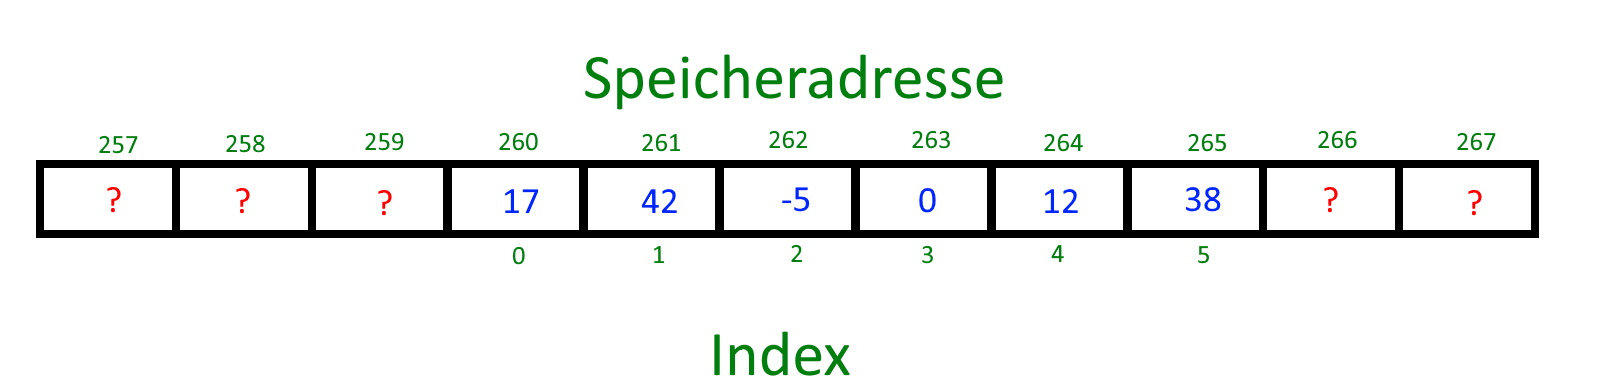
\includegraphics[width=\textwidth]{graph/Array_base}
	\end{figure}
\end{frame}

\begin{frame}{Grundoperationen}{Anlegen eines Arrays}
	\begin{itemize}
		\item Bei Anlegen eines Arrays muss immer die Größe festgelegt werden
		\item Vorher können keine Elemente hinzugefügt bzw. manipuliert werden
		\item Bei Initialisierung des Arrays wird ein Speicherbereich für dieses reserviert
		\item Größe des Speicherbereichs für ein Array der Größe $N$ ergibt sich aus:
	\end{itemize}
	$Speicher_{Byte}=ElementSize_{Byte}\cdot N$
\end{frame}

\begin{frame}{Grundoperationen}{Zugriff auf Elemente}
	\begin{itemize}
		\item Zugriffe auf Listenelemente passieren immer in konstanter Zeit
		\item Dadurch ergibt sich die Komplexität zu: $O(1)$
		\item Begründung:
		\begin{itemize}
			\item Elemente liegen "`hintereinander"' im Speicher $\rightarrow$ Haben fortlaufende Speicheradressen
			\item Die Adresse des ersten Elements ist immer bekannt
			\item Heißt, bei Abrufen des $n$-ten Elements muss von der Startadresse nur eine bestimmte Schrittzahl addiert werden
			\item Jeder Zugriff auf ein Element ist somit (auf unterster Ebene) eine Addition und eine Leseoperation
		\end{itemize}
	\end{itemize}
\end{frame}


\begin{frame}{Graphische Darstellung}{Zugriff auf Elemente}
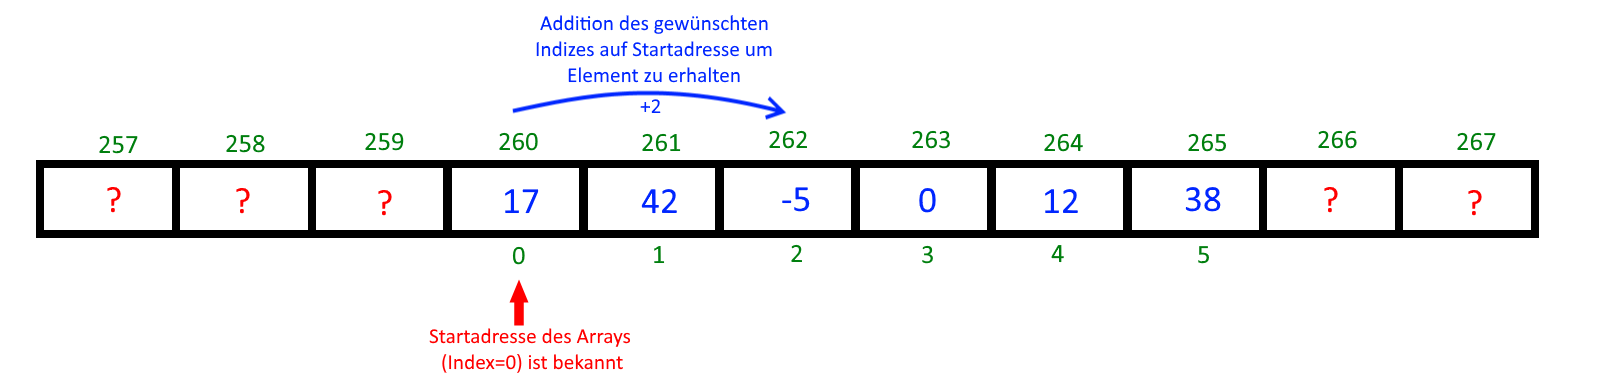
\includegraphics[width=\textwidth]{graph/array_access}
\end{frame}

\begin{frame}{Grundoperationen}{An-/Einfügen von Elementen}
	\begin{itemize}
		\item Nachträgliches Einfügen von Elementen ist nicht trivial
		\item Grund dafür ist die Speicherstruktur von Arrays
		\item Dadurch, dass die Elemente fortlaufend im Speicher liegen...
		\begin{itemize}
			\item ...müsste bei Einfügen sichergestellt sein, dass der nachfolgende Speicher noch nicht genutzt ist (Was meist nicht der Fall ist)
			\item ...und alle Elemente die nach dem eingefügten Element liegen, nach rechts "`verschoben"' werden
		\end{itemize}
		\item Dadurch häufig das anlegen eines neuen Arrays nötig
		\item Und das ausführen von vielen Kopieroperationen
	\end{itemize}
\end{frame}

\begin{frame}{Einfügen in Arrays}{Visualisiert}
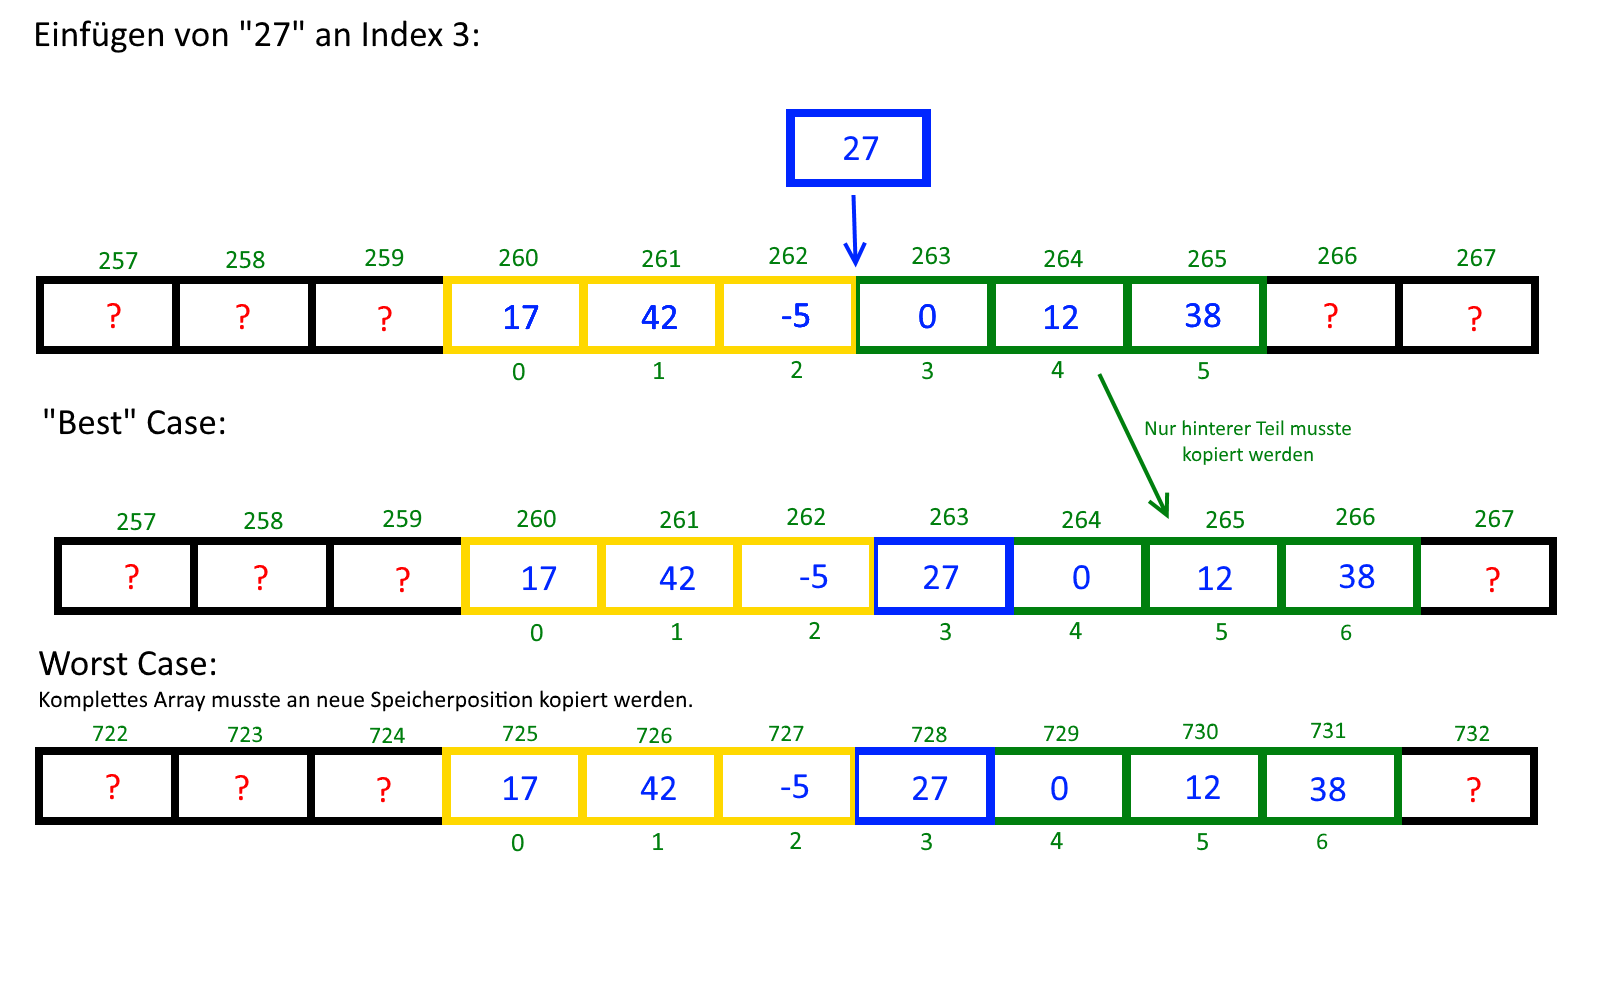
\includegraphics[height=6cm]{graph/array_insert}
\end{frame}

\begin{frame}{Komplexität}{Beim einfügen}
	\begin{itemize}
		\item Theoretischer Best-Case:
		\begin{itemize}
			\item Einfügen am Ende des Arrays
			\item ...solange der nachfolgende Speicher noch ungenutzt ist
			\item Dann wäre lediglich eine Kopieroperation erforderlich
		\end{itemize}
		\item In der Regel kann jedoch davon ausgegangen werden, dass...
		\begin{itemize}
			\item ...ein neues Array (an einem anderen Speicherbereich) angelegt werden muss
			\item ...und jedes Element des Arrays kopiert werden muss
		\end{itemize}
		\item Komplexität ergibt sich hierbei zu: $O(N)$
	\end{itemize}
\end{frame}

\begin{frame}{Ermitteln der Länge}{In Arrays}
	\begin{itemize}
		\item Bestimmen der Elemente eines Arrays nicht trivial möglich
		\item Da Array nur einen Speicherbereich beschreibt und seine eigene Größe nicht kennt
		\item Zählen von Elementen nicht möglich, da Abbruchbedingung nicht bekannt
		\item Größe muss somit selbst gespeichert und verwaltet werden
		\begin{itemize}
			\item Passiert in Java automatisch
			\item Da ein Array auch immer ein Objekt ist
			\item Bestimmen der Größe über das \texttt{length} Attribut
		\end{itemize}
	\end{itemize}
\end{frame}

\begin{frame}{Entfernen von Elementen}{In Arrays}
	\begin{itemize}
		\item Entfernen führt zu Problem im Speicherbereich:
		\item Durch das Entfernen würde eine "`Lücke"' im Array entstehen
		\item Daten im Array müssen jedoch fortlaufenden Speicher belegen
		\item D.h., Alle Elemente hinter dem entfernten Element müssen eine Position nach links verschoben werden
		\begin{itemize}
			\item "`Teure"' Kopiervorgänge nötig
		\end{itemize}
		\item Komplexität ergibt sich somit zu $O(N)$ (Worst-Case)
	\end{itemize}
\end{frame}

\begin{frame}{Entfernen von Elementen}{Visualisiert}
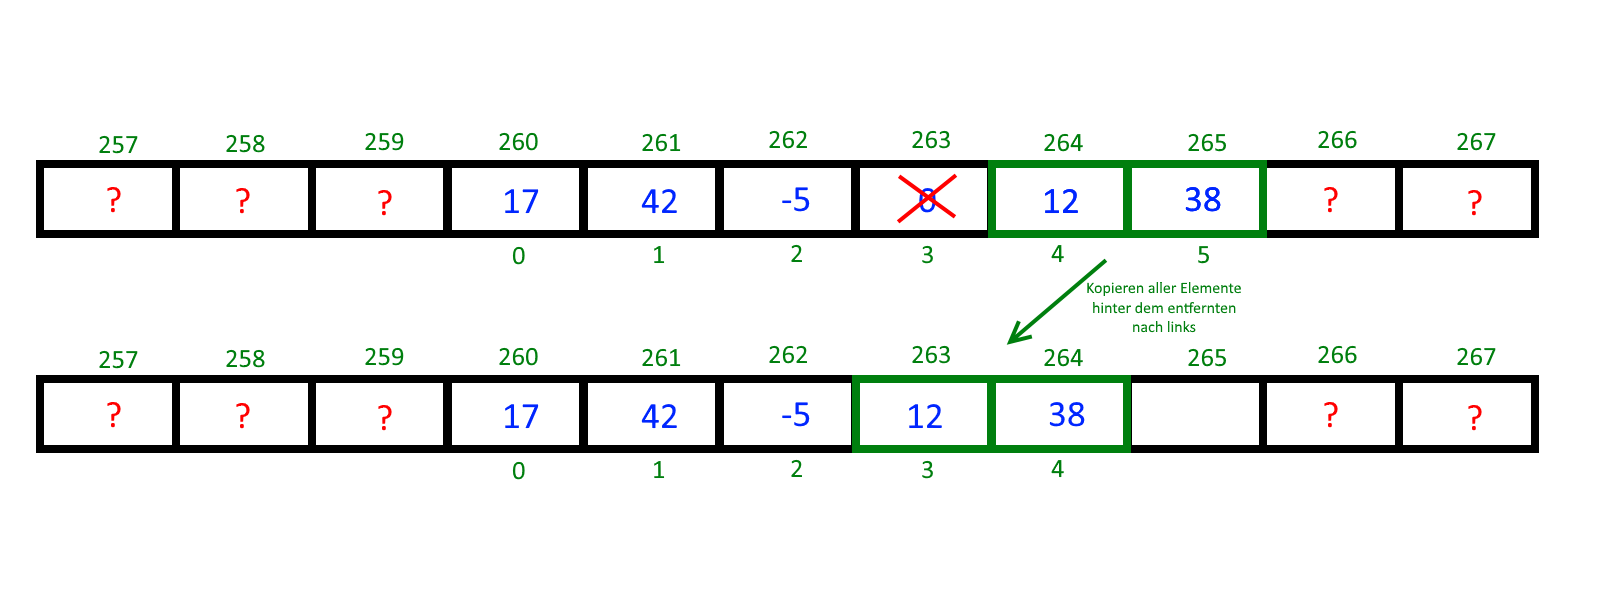
\includegraphics[width=\textwidth]{graph/array_remove}
\end{frame}

\begin{frame}{Entfernen von Elementen}{Weitere Aspekte}
	\begin{itemize}
		\item Beim entfernen von Elementen wird hinten Speicher "`frei"'
		\item Dieser ist (technisch) noch dem Array zugeordnet
		\begin{itemize}
			\item Heißt: Größe des Arrays muss theoretisch aktualisiert werden (Wenn man diese manuell verwalten muss)
		\end{itemize}
		\item Freigewordener Speicher kann jedoch später wiederverwendet werden:
		\begin{itemize}
			\item Elemente können theoretisch hinzugefügt werden ohne, dass das Array vergrößert werden muss
			\item Dafür müssen dann jedoch zwei Werte getracked werden:
			\item Die reservierte Größe des Arrays
			\item Die aktuell genutzte Größe des Arrays
			\item \texttt{ArrayList} Implementierung arbeitet ähnlich
		\end{itemize}
	\end{itemize}
\end{frame}

\begin{frame}{Konkatinieren von Arrays}
	\begin{itemize}
		\item Beim kombinieren zweier Arrays ergibt sich ähnliches Problem wie beim Einfügen
		\item Array hat ggf. nicht genug Platz um Elemente von beiden Arrays aufzunehmen
		\item Daher sind meist folgende Schritte nötig um zwei Arrays mit Länge $N$ und $M$ zu kombinieren:
		\begin{itemize}
			\item Anlegen eines neues Arrays mit Größe $N+M$
			\item Kopieren aller Elemente des ersten Arrays in den vorderen Teil
			\item Kopieren aller Elemente des zweiten Arrays in den hinteren Teil
		\end{itemize}
		\item Dadurch ergibt sich die Komplexität zu $O(N+M)$ (inklusive Overhead für Anlegen des neuen Arrays)
	\end{itemize}
\end{frame}

%\begin{frame}{Vor- und Nachteile}
%\end{frame}
	
	\outlineFrame{Linked Lists}
	\begin{frame}{Allgemeines}{Über Linked Lists}
	\begin{itemize}
		\item Simple Listenstruktur
		\item Elemente können verteilt im Speicher liegen
		\item Jedes Element speichert einen Datenwert
		\item ...und eine Referenz zum Nachfolger
		\item Speichern mehrdimensionaler Daten theoretisch möglich
		\begin{itemize}
			\item Wenn der Datenwert auch wieder eine Linked List ist
			\item Zugriff allerdings weniger intuitiv als im Array
		\end{itemize}
	\end{itemize}
\end{frame}


\begin{frame}{Eigenschaften}{Von Linked Lists}
	\begin{itemize}
		\item Muss keinen fortlaufenden Teil im Speicher belegen
		\item Dadurch entfallen einige Nachteile des Arrays:
		\begin{itemize}
			\item Größe muss nicht bei Initialisierung bekannt sein
			\item Liste kann dynamisch wachsen bzw. schrumpfen (Ohne "`teuere"' Kopiervorgänge)
			\item Einfügen bzw. Entfernen ist schneller
		\end{itemize}
		\item Allerdings ist der Zugriff auf Elemente langsamer
	\end{itemize}
\end{frame}

\begin{frame}{Datenstruktur von Linked Lists}{Listenelemente}
	\begin{itemize}
		\item Jedes Element einer Linked List ist ein Objekt
		\item Jedes Objekt vom Typ \textit{ListElement} besteht aus:
		\begin{itemize}
			\item Einem Member das den Wert des aktuellen Elements speichert. Datentyp ist der Typ, den die Liste speichert (\texttt{Double}, \texttt{Integer} etc.)
			\item Einem Member welches das nächste Element (bzw. eine Referenz darauf) in der Liste repräsentiert. Datentyp ist hier \texttt{ListElement}
		\end{itemize}
		\item Gibt es kein nächstes Element in der Liste kann dies über ein spezielles \texttt{tail} Objekt oder eine \texttt{null} Referenz dargestellt werden
	\end{itemize}
\end{frame}

\begin{frame}{Datenstruktur von Linked Lists}{Liste}
	\begin{itemize}
		\item Die Liste vom Typ \texttt{LinkedList} besteht an sich lediglich aus:
		\begin{itemize}
			\item Einem Member \texttt{head}(Auch: \texttt{first}, \texttt{top} o.Ä.) vom Typ \texttt{ListElement}, welches das erste Element der Liste repräsentiert.
			\item Den für die Liste benötigten Operationen zum Zugriff und Manipulation von Listenelementen
		\end{itemize}
		\item Sollte die Liste leer sein, so ist \texttt{head} ein Verweis auf \texttt{null} oder ein spezielles Element, das das Ende einer Liste repräsentiert.
	\end{itemize}
\end{frame}

\begin{frame}{Datenstruktur von Linked Lists}{Visualisiert}
%TODO: Visualisierung LinkedLists
\end{frame}

\begin{frame}{Grundoperationen}{Anlegen einer Linked List}
	\begin{itemize}
		\item Bei Anlegen einer neuen Linked List wird diese als leere Liste initialisiert
		\item Anders als beim Array muss kein Speicher für die Listenelemente reserviert werden
		\item Das heißt, das \texttt{head} Element wird mit einer \texttt{null} Referenz initialisiert
		\item Das erste Element, das hinzugefügt wird, wird automatisch zum \texttt{head} Elemente der Liste
		\item Wird ein Element hinzugefügt, wird erst zum Zeitpunkt des Hinzufügens der Speicher für dieses Element reserviert
	\end{itemize}
\end{frame}

\begin{frame}{Grundoperationen}{Zugriff auf Elemente}
	\begin{itemize}
		\item Zugriff auf Elemente muss immer sequentiell vom \texttt{head} Element aus erfolgen
		\item Zugriff auf das $n$-te Element erfolgt durch wiederholtes Zugreifen auf das \texttt{next} Element
		\item Bedeutet:
		\begin{itemize}
			\item Je weiter hinten das gesuchte Element steht, desto mehr Operationen sind möglich
			\item Somit ergibt sich die Komplexität zu $O(N)$
		\end{itemize}
	\end{itemize}
\end{frame}

\begin{frame}[fragile]{Zugriff auf Listenelemente}{Mögliche Codeimplementierung}
\lstset{style=java}
\begin{lstlisting}
public T getElement(int index){
	ListElement res = head;
	for(int i=0;i<index;i++){
		res = res.getNext();
	}
	return res.getValue();
}
\end{lstlisting}
\end{frame}
	
	\outlineFrame{Double Linked Lists}
	\begin{frame}
\end{frame}
	
	%\outlineFrame{Aufgaben I}
	\begin{frame}{Aufgabe 1}{ArrayList}
Im ersten Teil haben wir über die Eigenschaften von Arrays gesprochen. Unter anderem ging es darum, 
dass Arrays durch ihre Struktur relativ unflexibel sind, was das hinzufügen von Elementen betrifft.

Das \texttt{Collections} Interface bietet mit der \texttt{ArrayList} Klasse eine Liste an, die im Hintergrund
ein Array zum speichern von Daten anbietet. Diese Liste bietet die zwei Funktionen \texttt{size()} und \texttt{capacity} an.
\begin{enumerate}
	\item Untersucht den Unterschied zwischen den beiden Funktionen
	\item Untersucht, wie sich die Ergebnisse der beiden Funktionen verhalten, wenn Elemente hinzugefügt und entfernt werden
	\item Welche Rückschlüsse lassen sich daraus über die Datenorganisation der ArrayList treffen?
\end{enumerate}
\end{frame}

\begin{frame}{Aufgabe 2}{Linked List}
	\begin{enumerate}
		\item Entwerft eine \texttt{LinkedListElement<T>} Klasse mit den in der Vorlesung vorgestellten Eigenschaften
		\item Entwerft eine \texttt{LinkedList<T>} Klasse, die zur Speicherung der Daten die \texttt{LinkedListElement<T>} Klasse verwendet. Die Liste sollte folgende Funktionen integrieren:
		\begin{itemize}
			\item \texttt{get(int index)} - Gibt das Element an einem bestimmten Index zurück
			\item \texttt{size()} - Gibt die Anzahl der Elemente in der Liste zurück
			\item \texttt{insert} - Fügt ein bestimmtes Element an einem gegebenen Index ein
			\item \texttt{remove(index i)} - Entfernt das Element an dem gegebenen Index
		\end{itemize}
	\end{enumerate}
\end{frame}

\begin{frame}{Aufgabe 3}{Double Linked List}
Entwerft analog zu Aufgabe 2 die Klasse \texttt{DoubleLinkedListElement<T>} und \texttt{DoubleLinkedList<T>}
\end{frame}
	
	\outlineFrame{Stacks}
	\begin{frame}{Allgemeines}{Zu Stacks}
	\begin{itemize}
		\item "`Stapel"' $\rightarrow$ Beschreibt Funktionsweise sehr passend
		\item Listenstruktur in der nur Zugriff auf das "`oberste"' Element möglich ist
		\item Oberstes Element ist hier das zuletzt hinzugefügte
		\item Daten werden intern (als private Variable) verwaltet
		\begin{itemize}
			\item z.B. als Array oder Linked List
		\end{itemize}
	\end{itemize}
\end{frame}

\begin{frame}{Allgemeines}{Formale Definition Stack (Vgl. \cite{fahr:list})}
	\begin{alertblock}{Definition Stack}
	Ein Stack lässt sich \textbf{rekursiv} definieren. Zu jedem Zeitpunkt ist ein Stack entweder:
	\begin{itemize}
		\item Eine leere Datenstruktur
		\item Bestehend aus einem obersten Element und dem Rest, wobei der Rest wieder ein Stack ist
	\end{itemize}
	\end{alertblock}
\end{frame}

\begin{frame}{Allgemeines}{Stack Interface (Vgl. \cite{stacksqueues})}
	\begin{itemize}
		\item Grundlegendes Interface besteht aus zwei Operationen:
		\begin{itemize}
			\item \texttt{push} - Fügt ein Element hinten an den Stack an
			\item \texttt{pop} - Gibt das oberste Elemente des Stacks zurück und entfernt dieses aus dem Stack
		\end{itemize}
		\item Außerdem in der Regel noch Teil des Interfaces:
		\begin{itemize}
			\item \texttt{peek} - Gibt das oberste Element zurück, ohne es zu entfernen
			\item \texttt{isEmpty}
		\end{itemize}
	\end{itemize}
\end{frame}

\begin{frame}{Grundoperationen}{Anlegen eines Stacks}
	\begin{itemize}
		\item Stack wird als leere Datenstruktur initialisiert
		\item Je nachdem wie die Daten intern strukturiert sind muss ggf. eine Größe initialisiert werden
		\item Sobald das erste Element hinzugefügt wird, wird dieses zum obersten (\texttt{top}) Element
	\end{itemize}
\end{frame}

\begin{frame}{Grundoperationen}{Zugriff auf Elemente}
	\begin{itemize}
		\item Zugriff nur auf das letzte Element der Liste (Zletzt hinzugefügt)
		\item \texttt{pop} gibt das letzte Element zurück und entfernt dieses aus der Liste
		\item \texttt{peek} Gibt das letzte Element zurück ohne es zu entfernen
		\begin{itemize}
			\item Wiederholte Zugriffe auf \texttt{peek} geben also immer das gleiche Ergebnis zurück (Sofern der Stack zwischenzeitlich nicht manipuliert wurde)
		\end{itemize}
		\item Zugriff auf beliebige Elemente im Stack nicht möglich (Zuminndest sollte der Stack dafür kein Interface anbieten)
	\end{itemize}
\end{frame}

\begin{frame}{Grundoperationen}{An-/Einfügen von Elementen}
	\begin{itemize}
		\item Hinzufügen nur für das Ende des Stacks vorgesehen
		\item Dafür ist die Komplexität $O(1)$
		\item Hinzufügen in der Mitte des Stacks nicht vorgesehen
		\begin{itemize}
			\item Daher sehr aufwändig
			\item Es müssen von hinten sukzessiv Elemente entfernt werden, bis der gewünschte Index die letzte Position des Stacks wäre
			\item Dann wird das neue Element hinzugefügt
			\item Dann müssen alle zuvor entfernten Elemente wieder hinzugefügt werden
			\item Diese Operation sollte aber \textbf{nicht} Teil des Stack Interfaces sein
		\end{itemize}
	\end{itemize}
\end{frame}

\begin{frame}{Grundoperationen}{Bestimmen der Größe}
	\begin{itemize}
		\item Größe des Stacks wird in der Regel parallel verwaltet
		\item Und bei Aufrufen von \texttt{push} und \texttt{pop} aktualisiert
		\item Sonst wäre zum zählen folgendes Vorgehen nötig:
		\begin{itemize}
			\item Kopiere den Stack
			\item Entferne aus dem kopierten Stack solange Elemente bis der Stack leer ist
			\item Bei jedem entfernen erhöhe einen Zähler um 1
		\end{itemize}
	\end{itemize}
\end{frame}

\begin{frame}{Grundoperationen}{Entfernen von Elementen}
	\begin{itemize}
		\item Stack Interface bietet nur Möglichkeit, letztes Element zu entfernen
		\item Über die \texttt{pop} Funktion
		\item Entfernen in der Mitte vom Stack nicht möglich
		\begin{itemize}
			\item Kann theoretisch durch einen Benutzer realisiert werden (Ähnliches Vorgehen wie beim Einfügen in der Mitte)
			\item Sollte jedoch nicht Teil des Interfaces sein
		\end{itemize}
	\end{itemize}
\end{frame}

\begin{frame}{Grundoperationen}{Konkatinieren von Stacks}
	\begin{itemize}
		\item Kombinieren von zwei Stack relativ aufwendig
		\item Wenn das Ende des zweiten Stacks auch das Ende des zusammengefügten Stacks sein sollte
		\item Denn: Bei entfernen aller Elemente vom Stack wird die Reihenfolge der Elemente invertiert
		\item Nötiges Vorgehen:
		\begin{itemize}
			\item Entferne über \texttt{pop} sukzessive die Elemente vom zweiten Stack bis dieser leer ist und füge sie (über \texttt{push}) zu einem temporären Stack hinzu
			\item Entferne sukzessive die Elemente vom temporären Stack und füge sie an den ersten Stack an
		\end{itemize}
	\end{itemize}
\end{frame}

\begin{frame}{Anwendungsfälle}{Für Stacks}
	\begin{itemize}
		\item Backtracking Algorithmen - Jeder Schritt wird auf dem Stack gespeichert und kann über den Stack "`zurückgegangen werden"'
		\begin{itemize}
			\item Beispiel: Labyrinth Algorithmus.
			\item Jeder Schritt wird auf einem Stack gespeichert
			\item Bei erreichen einer Sackgasse werden die zuletzt gemachten Schritte so lange zurück gegangen, bis ein anderer Schritt möglich ist
		\end{itemize}
		\item Rückgängig Funktion - Jede Aktion wird auf einem Stack abgelegt und kann somit rückgängig gemacht werden
	\end{itemize}
\end{frame}
	
	\outlineFrame{Queues}
	\begin{frame}{Allgemeines}{Zu Queues (Vgl. \cite{stacksqueues})}
	\begin{itemize}
		\item Funktionieren ähnlich wie Stacks
		\item Hier jedoch andere Zugriff:
		\begin{itemize}
			\item Elemente können nur hinten angefügt werden
			\item ...und vorn entfernt werden
		\end{itemize}
		\item Stellt eine "`Warteschlange"' dar
		\item Interne Datenstruktur wie beim Stack variabel
		\item Wichtig ist, dass von außen nur über das Queue Interface zugegriffen werden kann
	\end{itemize}
\end{frame}

\begin{frame}{Allgemeines}{Queue Interface (Vgl. \cite{stacksqueues})}
	\begin{itemize}
		\item Queue Interface besteht aus zwei grundlegenden Operationen:
		\begin{itemize}
			\item \texttt{enqueue} - Hängt ein Element hinten an die Queue an 
			\item \texttt{dequeue} - Gibt das ersten Element der Queue zurück und entfernt dieses
		\end{itemize}
		\item Wie im Stack gibt es meist noch weitere Hilfsfunktionen wie \texttt{isEmpty} oder \texttt{peek}
	\end{itemize}
\end{frame}

\begin{frame}{Grundoperationen}{An-/Einfügen von Elementen}
	\begin{itemize}
		\item Anfügen von Elementen nur am Ende möglich
		\item Einfügen in der Mitte nicht vorgesehen (In der Standardqueue)
		\item Um ein Element an der Stelle $i$ einzufügen müsste man:
		\begin{itemize}
			\item Die Größe der Queue bestimmen ($n$)
			\item Die ersten $i-1$ Elemente der Queue entfernen und direkt hinten anfügen
			\item Dann das einzufügende Element anhängen
			\item Dann die vordersten $n-i+1$ Elemente entfernen und direkt hinten anfügen
		\end{itemize}
		\item Solche Operationen sind jedoch nicht Teil des Standardinterfaces
	\end{itemize}
\end{frame}

\begin{frame}{Grundoperationen}{An-/Einfügen von Elementen}
	\begin{itemize}
		\item Es gibt Queues in denen neue Element nicht zwangsweise hinten angehängt werden
		\item Sondern nach anderen Kriterien in der Queue sortiert werden, z.B.
		\begin{itemize}
			\item Angegebener Priorität
			\item (Hash-)Wert des Elements
		\end{itemize}
		\item Wichtig hierbei: Das Interface sollte sich hierbei nach außen nicht maßgeblich verändern
		\item Die Logik wie das Element in die interne Struktur eingefügt wird, bleibt intern!
	\end{itemize}
\end{frame}

\begin{frame}{Grundoperationen}{Bestimmen der Größe}
	\begin{itemize}
		\item Wie auch im Stack ist die Größenbestimmung sehr aufwendig
		\item Kopieren der Queue und sukzessives entfernen notwendig
		\item Daher wird auch hier die Größe meist "`manuell"' verwaltet und beim Hinzufügen/Entfernen aktualisiert
	\end{itemize}
\end{frame}

\begin{frame}{Grundoperationen}{Entfernen von Elementen}
	\begin{itemize}
		\item Das Interface erlaubt nur das entfernen des vordersten Elements
		\item Um Elemente in der MItte zu entfernen müsste ähnlich vorgegangen werden wie beim Einfügen
		\item Auch hier gilt wieder: Das Entfernen "`in der Mitte"' sollte nicht Teil des Interfaces sein
	\end{itemize}
\end{frame}

\begin{frame}{Grundoperationen}{Konkatinieren von Queues}
	\begin{itemize}
		\item Kombinieren von Queues ist - vergleichsweise - "`simpel"'
		\begin{itemize}
			\item Im Grunde muss nur wiederholt das erste Element der zweiten Queue entfernt werden
			\item ...und direkt an die erste angefügt werden
		\end{itemize}
		\item Je nachdem wie die Queue intern strukturiert ist, kann dies über eine bereitgestellte "`append"' Funktion optimiert werden
		\begin{itemize}
			\item Zum Beispiel durch direktes zusammenfügen der internen Linked Lists
		\end{itemize}
	\end{itemize}
\end{frame}

\begin{frame}{Anwendungsfälle}{Für Queues}
	\begin{itemize}
		\item Scheduling von nacheinander ablaufenden Operationen
		\item Planung von Prozessen in gemeinsam genutzten Ressourcen
		\begin{itemize}
			\item Wenn eine Ressource gerade belegt ist und ein weterer Prozess sie aber benötigt
			\item Wird der Prozess zur nächsten Berechnung in der Queue gespeichert
		\end{itemize}
	\end{itemize}
\end{frame}
	
	\outlineFrame{Trees}
	\begin{frame}{Allgemeines}{Baumstrukturen}
	\begin{itemize}
		\item Unterscheiden sich von den bisherigen Strukturen
		\item Bisher hatte jedes Element einer Datenstruktur immer einen "`Nachfolger"'
		\item ...und einen Vorgänger
		\item Bäume können jedoch mehrere "`Nachfolger"' haben
		\begin{itemize}
			\item Man spricht in der Regel von \textbf{Knoten}
			\item Es gibt genau einen Knoten im Baum, der keinen Eingang ("`Vorgänger"') besitzt
			\begin{itemize}
				\item Dies ist der \textbf{Wurzelknoten} des Baumes
			\end{itemize}
			\item Alle anderen Knoten haben genau einen Eingang
		\end{itemize}
		\item In der Regel beschäftigt man sich hauptsächlich mit \textit{Binärbäumen}
		\begin{itemize}
			\item Diese haben \textbf{zwei} Nachfolger
		\end{itemize}
	\end{itemize}
\end{frame}

\begin{frame}{Allgemeines}{Definition von Bäumen}
	\begin{alertblock}{Graphentheoretische Definition}
	Ein Baum ist ein endlicher, schwach zusammenhängender gerichteter Graph, für dessen Knotenpunkte gilt:
	\begin{enumerate}
		\item Es gibt genau einen Knoten, der keinen Eingang hat (Wurzel des Baumes)
		\item Alle übrigen Knotenpunkte haben genau einen Eingang.
	\end{enumerate}
	\end{alertblock}
	
	\begin{alertblock}{Rekursive Definition(Binärbaum)}
	Eine Baumstruktur vom Grundtyp T ist:
	\begin{enumerate}
		\item Eine leere Struktur
		\item Ein Knoten vom Typ T mit genau zwei disjunkten Teilbäume vom Grundtyp T
	\end{enumerate}
	\end{alertblock}
\end{frame}

\begin{frame}{Allgemeines}{Struktur der Knoten im Baum}
	\begin{itemize}
		\item Grundsätzlich besteht ein Knoten(Im Binärbaum) aus drei Elementen
		\begin{itemize}
			\item Einem Schlüssel (=Datenwert) für den Knoten
			\item Einen linken Teilbaum
			\item Einen rechten Teilbaum
		\end{itemize}
	\end{itemize}
\end{frame}

\begin{frame}{Eigenschaften}{Von Binärbäumen}
	\begin{alertblock}{Vollständige Binärbäume}
	In einem Binärbaum kann jede Ebene maximal $2^{(Tiefe-1)}$ Knoten besitzen. Ein Binärbaum ist dann vollständig ausgeglichen, wenn auf jeder Ebene, mit Ausnahme der letzten, genau diese
	$2^{(Tiefe-1)}$ Knoten existieren und die Knoten auf der letzten Ebene soweit links wie möglich stehen
	\end{alertblock}
	
	\begin{alertblock}{Suchbaum}
	Wenn für alle Knoten K eines Baumes gilt, dass...
	\begin{enumerate}
		\item ...alle Schlüssel im linken Teilbaum von K kleiner...
		\item ...alle Schlüssel im rechten Teilbaum von K größer...
	\end{enumerate}
	... als der Schlüssel des Knotens K sind, so handelt es sich um einen Suchbaum
	\end{alertblock}
\end{frame}

\begin{frame}{Grundoperationen}{In Binärbäumen}
	\begin{itemize}
		\item Zur Vereinfachung betrachten wir für Binärbäume (Suchbäume) folgende Operationen:
		\begin{itemize}
			\item Einfügen von Elementen
			\item Entfernen von Elementen
			\item Bestimmen der Anzahl von Elementen
		\end{itemize}
		\item Grundoperationen basieren fast immer auf rekursivem Aufruf auf den Teilbäumen!
	\end{itemize}
\end{frame}

\begin{frame}{Grundoperationen}{Einfügen von Elementen}
	\begin{itemize}
		\item Für das Einfügen eines Elements $X$ in einen Baum $B$ werden vier Fälle unterschieden:
		\begin{itemize}
			\item Ist $B$ leer, so ist das Ergebnis der Baum mit dem Schlüssel $X$
			\item Ist $X$ identisch mit dem Schlüssel von $B$ so ist $X$ bereits im Baum und wird nicht hinzugefügt
			\item Ist $X$ kleiner als der Schlüssel von $B$ so füge $X$ im linken Teilbaum ein
			\item Ist $X$ größer als der Schlüssel von $B$ so füge $X$ im rechten Teilbaum ein
		\end{itemize}
	\end{itemize}
\end{frame}

\begin{frame}{Einfügen in Suchbäume}{Beispiele}
%TODO: Beispiele Einfügen
\end{frame}

\begin{frame}{Grundoperationen}{Entfernen aus Suchbäumen}
\begin{itemize}
	\item Beim Entfernen eines Elements mit dem Schlüssel $X$ können vier Fälle auftreten:
	\begin{itemize}
		\item Der Baum enthält $X$ nicht - Fertig.
		\item Der Knoten mit dem Schlüssel $X$ hat keinen Nachfolger - $X$ wird entfernt, Fertig.
		\item Der Knoten mit dem Schlüssel $X$ hat genau einen Nachfolger
		\item Der Knoten mit dem Schlüssel $X$ hat genau zwei Nachfolger
	\end{itemize}
\end{itemize}
\end{frame}

\begin{frame}{Entfernen}{$X$ hat einen Nachfolger}
	\begin{itemize}
		\item Simpler Fall
		\item Hier "`rutscht"' der Nachfolger (Gesamter Teilbaum) einfach an die Stelle des zu entfernenden Elements
		\item Keine weiteren Operationen - Fertig.
	\end{itemize}
\end{frame}

\begin{frame}{Entfernen}{Visualisiert für einen Nachfolger}
%TODO: Visualisierung Entfernen
\end{frame}

\begin{frame}{Entfernen}{$X$ hat zwei Nachfolger}
	\begin{itemize}
		\item Problematik: Welcher Nachfolger tritt an die Stelle von $X$
		\item ...damit die Suchbaumbedingung bestehen bleibt?
		\item Suchen des sogenannten \textbf{in-order Nachbarn} $N$ von $X$
		\begin{itemize}
			\item Ist das jeweils nächstgrößere bzw. -kleinere Element an $X$
			\item Also das kleinste ("`linkeste"') Element des rechten Teilbaums
			\item Oder größtes ("`rechteste"') Element des linken Teilbaums
		\end{itemize}
		\item $N$ tritt an die Stelle von $X$
		\item Teilbäume von $X$ bleiben (beinahe) unervändert
		\begin{itemize}
			\item Außer natürlich, dass $N$ aus dem Teilbaum entfernt wird
		\end{itemize}
	\end{itemize}
\end{frame}

\begin{frame}{Entfernen}{Visualisiert für zwei Nachfolger}
%TODO: Abbildung entfernen 
\end{frame}

\begin{frame}{Ausgeglichenheit}{Das Ying und Yang von Bäumen}
	\begin{itemize}
		\item Bisher können unsere (Teil-)Bäume verschiedene Tiefen haben
		\item Dies ist jedoch nicht optimal für z.B. Suchalgorithmen
		\item Die maximale Suchzeit lässt sich so nur schwer abschätzen
		\item Außerdem ist die durchschnittliche Suchzeit meist höher
		\item Daher:
		\begin{itemize}
			\item Definition eines Ausgeglichenheitskriteriums
			\item Dadurch Tiefe der Teilbäume ähnlich
			\item Führt zu besserer Performance bei Suchbäumen
		\end{itemize}
	\end{itemize}
\end{frame}

\begin{frame}{AVL Bäume}{Definition}
	\vfill
	\begin{alertblock}{Ausgeglichenheit nach AVL-Bedingung}
	Ein Baum ist dann ausgeglichen, wenn sich für jeden Knoten die Höhe der zugehörigen Teilbäume um
	höchstens 1 unterscheidet.
	\end{alertblock}
	\vfill
\end{frame}

\begin{frame}{AVL Bäume}{Visualisiert}
%TODO: Visualisierung Bäume
\end{frame}

\begin{frame}{Einfügen}{In AVL Bäume}
	\begin{itemize}
		\item Einfügen erfolgt vorerst nach normalem Verfahren von binären Suchbäumen
		\item Dadurch kann jedoch die AVL-Bedingung verletzt werden
		\item Dann muss der Baum wieder ausgeglichen werden
		\item Hierfür wird folgendermaßen vorgegangen:
		\begin{itemize}
			\item Wandere beginnend vo eingefügten Element $w$ nach oben
			\item Prüfe für jeden Knoten ob die AVL Bedingung verletzt ist
			\item Wenn ein Knoten $z$ gefunden wurde, für den die AVL-Bedingung verletzt wurde, gleiche den Baum aus
		\end{itemize}
	\end{itemize}
\end{frame}

\begin{frame}{Einfügen}{Ausgleichen von AVL Bäumen}
	\begin{itemize}
		\item Zum Ausgleichen von AVL-Bäumen gibt des die Links- bzw. Rechtsrotation
		\item Für einen unbalancierten Knoten $z$ sei:
		\begin{itemize}
			\item $y$ Der "`Kindknoten"' (Erste schritt) von $z$ auf dem Weg zum eingefügten Knoten $w$
			\item $x$ Der "`Enkelknoten"' (Zweite Schritt) von $z$ auf dem Weg zu $w$
		\end{itemize}
		\item Hier gibt es vier mögliche Fälle nach denen unterschiedlich rotiert werden muss:
		\begin{itemize}
			\item Links-Links
			\item Links-Rechts
			\item Rechts-Rechts
			\item Rechts-Links
		\end{itemize}
	\end{itemize}
\end{frame}

\begin{frame}{Links-Links}{Rechtsrotation}
%TODO: Visualisierung
\end{frame}

\begin{frame}{Rechts-Rechts}{Linksrotation}
\end{frame}

\begin{frame}{Links-Rechts}{Links-Rechts-Doppelrotation}
\end{frame}

\begin{frame}{Rechts-Links}{Rechts-Links-Doppelrotation}
\end{frame}
    
	%\outlineFrame{Aufgaben II}
	\begin{frame}{Aufgabe 1}
In der Vorlesung haben wir darüber gesprochen, dass die interne Datenstruktur von Queues und Stacks frei gewählt werden kann. Soo könnte beispielsweise
ein Array oder auch eine Linked List verwendet werden.
	\begin{itemize}
		\item Welche Vorteile ergeben sich aus dieser Austauschbarkeit der Datenstruktur?
		\item Ist die Verwendung eines simplen Arrays als Datenstruktur für eine Queue bzw. einen Stack sinnvoll?
		\begin{itemize}
			\item Welche Vor- und Nachteile der Array Struktur sollte man berücksichtigen?
		\end{itemize}
	\end{itemize}
\end{frame}

\begin{frame}{Aufgabe 2}
Entwerft und implementiert eine Klasse zum repräsentieren eines Stacks oder einer Queue. Die interne Datenstruktur kann von euch frei gewählt werden.

Die Klasse sollte mindestens die folgenden Methoden zur Verfügung stellen:
\begin{itemize}
	\item \texttt{isEmpty} - Gibt zurück, ob die Struktur leer ist
	\item \texttt{peek} - Gibt das vorderste (für Queues) bzw. letzte (für Stacks) zurück
	\item \texttt{clear} - Entfernt alle Elemente aus der Datenstruktur
	\item \texttt{size} - Gibt die Anzahl der Elemente zurück
	\item Sowie die entsprechenden Operationen zum hinzufügen bzw. entfernen
\end{itemize}
\end{frame}

\begin{frame}{Aufgabe 3}
In der Vorlesung haben wir über binäre Suchbäume gesprochen. 
	\begin{itemize}
		\item Zeichnet den entstehenden Baum, wenn ihr nacheinander die Elemente $(47. 63. 25. 13. 57. 18. 99. 14. 22. 37. 24. 28. 30.)$ hinzufügt.
		\item Wie sieht der resultierende Baum aus, wenn ihr das Element $13$ entfernt?
		\item Wie sieht der Baum aus, wenn ihr weiterhin das Element $25$ entfernt
	\end{itemize}
\end{frame}

\begin{frame}{Aufgabe 4}
Mithilfe von ausgeglichenen Bäumen kann die Suchzeit in Binärbäumen optimiert werden. Eine Möglichkeit zur Erstellung eines ausgeglichenen Baumes stellt die
AVL Bedingung dar. Durch diese wird sichergestellt, dass sich die Tiefen der Teilbäume zu jedem Zeitpunkt um maximal 1 unterscheiden.

\begin{itemize}
	\item Fügt in der gegebenen Reihenfolge die Elemente in einen intial leeren Binärbaum ein: $3.2.1.4.5.6.7.16.15$
\end{itemize}
\end{frame}
	
    \printbibliographyframe
    
	\section*{Kontakt}
	\begin{frame}{Kontakt}{}
	\begin{itemize}
		\item E-Mail: \href{mailto:lukas.abelt@airbus.com}{lukas.abelt@airbus.com}
		\item GitHub: \url{https://www.github.com/LuAbelt}
		\item GitLab: \url{https://www.gitlab.com/LuAbelt}
		\item Telefon(Firma): 07545 - 8 8895
		\item Telegram: LuAbelt
	\end{itemize}
\end{frame}
	

\end{document}